Для начала мы преобразуем изображение в черно-белое.

\begin{figure}[ht!]
    \centering
    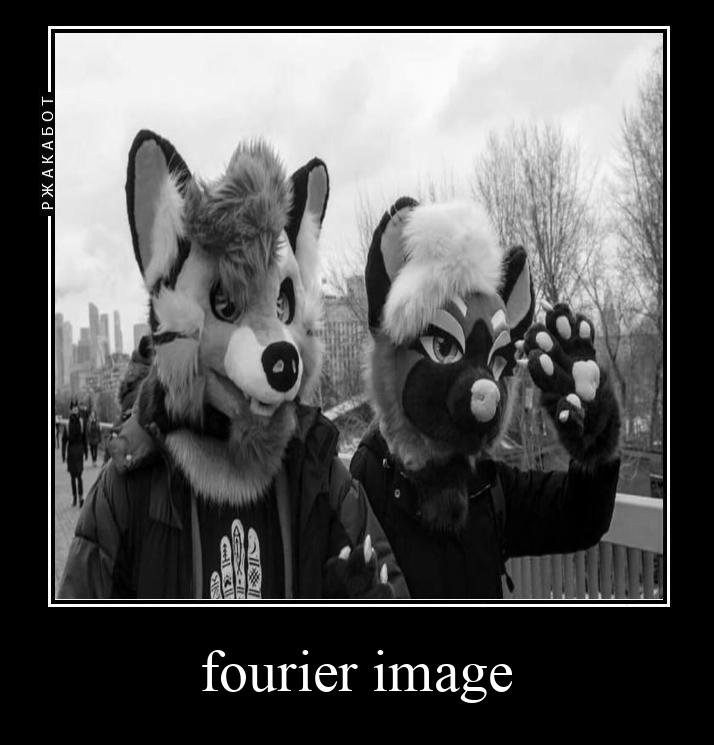
\includegraphics[width=0.5\textwidth]{/Users/nikolajprovorov/Yandex.Disk-368690@edu.itmo.ru.localized/Lab6_Furry_series/bw.png}
    \caption{Черно-белое изображение}
\end{figure}

Зададим матрицу ядра увеличния резкости:

\begin{equation}
    K = 
    \begin{bmatrix}
        0 & -1 & 0 \\
        -1 & 5 & -1 \\
        0 & -1 & 0
    \end{bmatrix}
\end{equation}

Посмотрим на результат применения:

\clearpage

\begin{figure}[ht!]
    \centering
    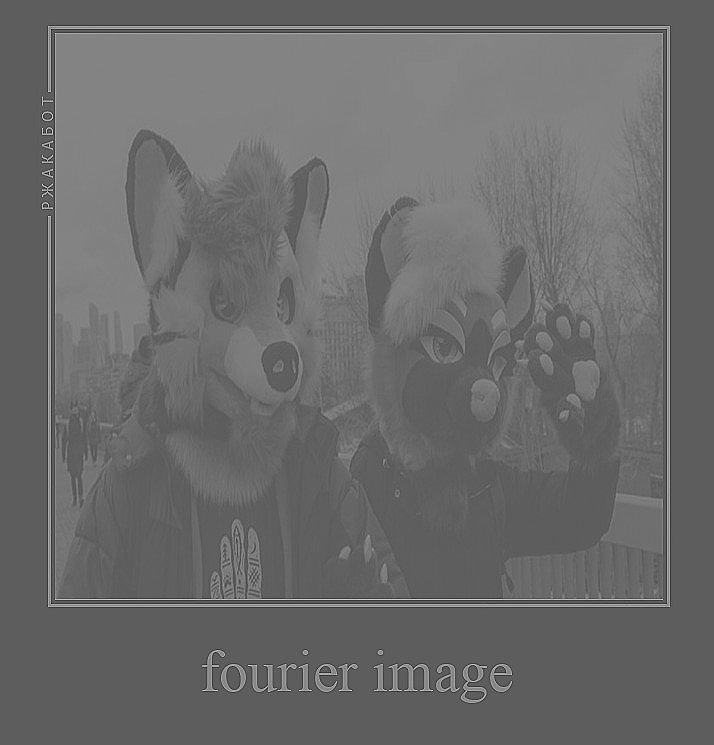
\includegraphics[width=0.5\textwidth]{/Users/nikolajprovorov/Yandex.Disk-368690@edu.itmo.ru.localized/Lab6_Furry_series/laplacian.png}
\end{figure}

Стало явно лучше, резкость увеличилась, но изображение потеряло в контрасте.

Давайте посмотрим теперь на результат всего вот того фурье:

\begin{figure}[ht!]
    \centering
    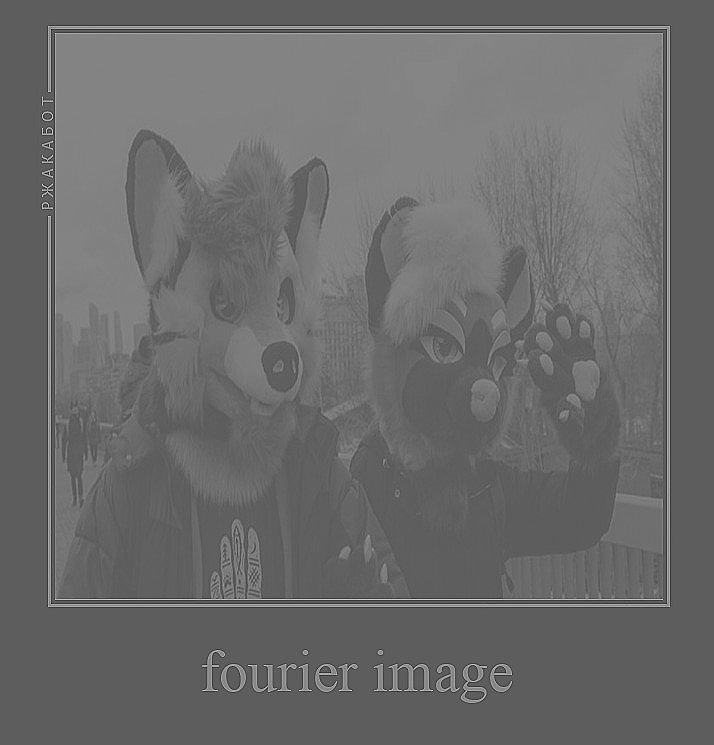
\includegraphics[width=0.5\textwidth]{/Users/nikolajprovorov/Yandex.Disk-368690@edu.itmo.ru.localized/Lab6_Furry_series/laplacian.png}
    \caption{Увеличение резкости изображения что-то там фурье}
\end{figure}

О, прикол, совпали. Теорема о свертке работает корректно.